\section{WebIDL Bindings} % (fold)
\label{sec:webidl_bindings}

In order to automatically generate stubs for JavaScript and C++ that allows communication between the two languages, an independent language, WebIDL, is used to define types and interfaces which will be used by both JavaScript and C++.

\begin{figure}
    \centering
    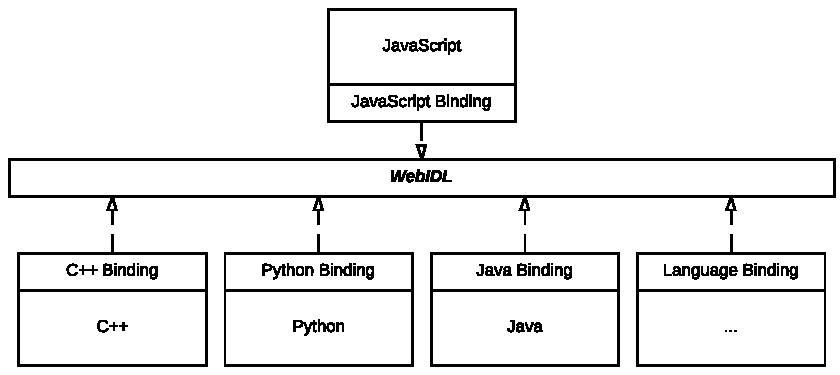
\includegraphics[width=1\textwidth]{JavaScript-WebIDL.pdf} 
    \caption{The WebIDL interface}
    \label{fig:webidl_intreface}
\end{figure}

The reason why this is needed is because JavaScript and C++ have entirely different type systems, and because the communication is two-way, we can't simply map a C++ type into a JavaScript type. Moreover, if the RPC framework were to be completely language independent, we would need a mapping between every languages type into a JavaScript type. Therefore, to generalise, WebIDL gives an intermediary type interface so that other languages can communicate with JavaScript. The WebIDL types and syntax is defined as a standard, and gives EcmaScript bindings. In other words, the conversion between WebIDL and JavaScript types is defined in the standard. It is then up to the developer of the other language to define a binding from that language to WebIDL. This is illustrated in Figure \ref{fig:webidl_intreface}.

In this section, we mention the C++ WebIDL bindings used in the Native Calls project, and the design decisions behind them.

The implementation challenges involved in implementing these bindings are discussed at a later chapter.

\subsection{Modules, Interfaces, and Functions} % (fold)
\label{sub:modules_and_interfaces}
In Native Calls, we make a distinction between `modules' and `interfaces'. Essentially, a module contains several interfaces. And an interface contains several function definitions.

When we define a module, we must define all the interfaces, type definitions, and dictionaries for it in the same generator call. The definitions could be in different IDL files.

In JavaScript, a module is represented as an object which has a property for each interface that module defines. Then, each interface has a property for each function that interface defines. 

In C++, a module is represented as a class, which sets up the module. When setting up the module, each function interface is added. An IDL interface is represented by a C++ header file. The header file defines each function that is in the interface.

% subsection modules_and_interfaces (end)

\subsection{Number and String Types} % (fold)
\label{sub:number_types}
WebIDL defines a number of numeric types, and also provides the JavaScript bindings for each type. The table below (TODO: give ref) shows the numeric types and their bindings in C++.

\begin{table}[h]
\begin{tabular}{l|lll}
\textbf{WebIDL Type} & \textbf{Min int} & \textbf{Max int} & \textbf{C++ Type}  \\ \hline
byte                 & $-2^{7}$         & $2^{7}-1$        & int8\_t            \\
octet                & $0$              & $2^{8}-1$        & uint8\_t           \\
short                & $-2^{15}$        & $2^{15}-1$       & int16\_t           \\
unsigned short       & $0$              & $2^{16}-1$       & uint16\_t          \\
long                 & $-2^{31}$        & $2^{31}-1$       & int32\_t           \\
unsigned long        & $0$              & $2^{32}-1$       & uint32\_t          \\
long long            & $-2^{63}$        & $2^{63}-1$       & int64\_t           \\
unsigned long long   & $0$              & $2^{64}-1$       & uint64\_t          \\
float                &                  &                  & float              \\
double               &                  &                  & double           
\end{tabular}
\end{table}

It can be observed that the integer types are represented in C++ with the size information in it, even though C++ has equivalent type names for each of the WebIDL integer types. For example, C++ supports the \lstinline{short} type, but we explicitly decide to represent \lstinline{short} as \lstinline{int16_t}. The reason why explicit size information is included in the type is because of different implementations of certain types. For example, depending on the C++ standard library implementation we use, a \lstinline{long} can be represented in 32 bits or 64 bits. But because WebIDL explicitly defines the actual size of the integer types, to stick to the standard, we can't tolerate this variation. For this reason, we use the explicit size types as shown above. This issue does not arise for \lstinline{float} and \lstinline{double} types as both C++ and JavaScript adhere to the IEEE 754 format.

Another interesting issue to note is that the bindings for large number types, such as \lstinline{long long}, are represented in JavaScript by the \emph{closest} numeric value. But because all JavaScript numbers are represented by 64 bit IEEE 754 (`double') types, the largest number that can be represented in JavaScript is actually $2^{53}-1$. This means that often the conversion between the WebIDL type and the JavaScript binding is \emph{lossy}, in the sense that it is not a one-to-one mapping. Although it would have been possible to overcome this issue by creating or using JavaScript `BigNumber' library classes, I decided to adhere to the specification, using the lossy conversion. This was for a couple of reasons:

\begin{itemize}
	\item Forcing the JavaScript user to use a number library is bad, as it adds more dependencies and is not conventional JavaScript e.g. the BigNumber library will have a different API to normal JavaScript numbers, and certain operations, such as addition, will not work properly.
	\item Using a different implementation, the RPC library could represent all data as \emph{binary}. JavaScript supports binary data in the form of ArrayBuffers.
	\item It is fairly unlikely that the developer would want to send back such large numbers to the JavaScript, and since the developer is developing for the web platform, they should be aware of JavaScript's limitations - including numeric type support.
\end{itemize}

To represent string types, the \lstinline{DOMString} WebIDL type is converted to the JavaScript \lstinline{string} type, as defined in the standard. As for the C++ binding, the \lstinline{std::string} class was chosen to represent DOMString. The alternative was to represent strings as character array buffers (\lstinline{char[]}). I decided to use the \lstinline{std::string} class for the following reasons:

\begin{itemize}
	\item JavaScript uses unicode (utf8) for strings. The developer would need to do some encoding/decoding to handle unicode characters, which might not fit in a byte.
	\item Simplicity: The PPAPI supports an \lstinline{AsString()} method on \lstinline{pp::Var} objects, which extracts the string value as a \lstinline{std::string} object.
	\item C++ developers use \lstinline{std::string} when they can. \lstinline{std::string} allows conversion to C strings using the \lstinline{c_str()} method.
\end{itemize}

% subsection number_types (end)

\subsection{Dictionary Types} % (fold)
\label{sub:dictionary_types}
The WebIDL standard defines the binding of a WebIDL dictionary to be a JavaScript Object with the keys being the identifier names of each dictionary member, and values being of the member's type. For example, Listing \ref{code_webidl_dictionary_example} shows an example of a dictionary definition in WebIDL and the corresponding JavaScript object according to the specification.

\lstset{language=C,caption={A WebIDL dictionary and its JavaScript binding},label=code_webidl_dictionary_example}
\begin{code}
// WebIDL
dictionary myObject {
  double id;
  DOMString name;
};

// Example JavaScript object
var myObj = {
  id: 31,
  name: "John Smith"
}
\end{code}

When a JavaScript object (and therefore a WebIDL dictionary) is sent to the NaCl module, it is represented in PPAPI as a \lstinline{pp::VarDictionary} object. \lstinline{pp::VarDictionary} allows extracting keys and values as \lstinline{pp::Var}. See background section \ref{sub:using_PPAPI} on page \pageref{sub:using_PPAPI} for more details.

We now consider how we can represent dictionaries in C++. The obvious approach is to represent a dictionary as a C \lstinline{struct}. The fields of the struct will have corresponding names and types as defined in the dictionary. For example, the struct shown in Listing \ref{code_webidl_struct_example} corresponds to the dictionary shown earlier in Listing \ref{code_webidl_dictionary_example}.


\lstset{language=C,caption={A C struct corresponding to the dictionary definition in Listing \ref{code_webidl_dictionary_example}},label=code_webidl_struct_example}
\begin{code}
struct myObject {
  double id;
  std::string name;
}

// example use
struct myObject myObj;
myObj.id = 31;
myObj.name = "John Smith";
\end{code}


The advantage of this is that the object passed to the C++ programmer will be a normal C++ struct. However, it will impact performance, since each field of the struct will need to be individually converted. In fact, this makes marshalling dictionaries the slowest conversion, according to the benchmarks (see section \ref{sec:performance_evaluation}, page \pageref{sec:performance_evaluation}).

However, other approaches are possible. One alternative is we could have simply passed the \lstinline{pp::VarDictionary} object to the developer, without modifying it. The advantage of doing this is that it will simplify the C++ RPC library and therefore make it faster to send and receive complicated structures. However, there are a few problems with this approach:

\begin{itemize}
	\item The C++ developer is now exposed to PPAPI. This adds a learning curve, as it is another library that the C++ developer would have to get used to in order to write their module.
	\item The C++ developer will need to do all the type marshalling by themselves. This renders the dictionary type definition that they wrote in WebIDL useless, and adds more burden on the developer.
	\item The use of \lstinline{pp::VarDictionary} is actually an implementation detail of the RPC library. In other words, we simply use this as a way of transporting the data from JavaScript to C++. Perhaps someone could write another implementation that uses full binary transfer for example, using Protocol Buffers (see background section \ref{sec:data_representation_and_transfer}, page \pageref{sec:data_representation_and_transfer}). In that case, passing the \lstinline{pp::VarDictionary} to the developer would actually be more burden on the library, and probably impact performance.
\end{itemize}

Another approach is to represent a dictionary as a \lstinline{std::map}. The advantage of this is that the map can be added to and deleted from dynamically and unlike structs, if a field is not specified, data is not allocated for it. The problem with \lstinline{std::map} however is that the keys and values of the map have strict types. If the values have the same type, then a map will do fine. But what about if the values have different types, such as in the example in Listing \ref{code_webidl_dictionary_example}? The only way around this is by using wrapper types. For example, using \lstinline{pp::Var} again to represent the actual value, so the \lstinline{std::map} will be from \lstinline{std::string} keys to \lstinline{pp::Var} values. But again, this means the developer will have to de-marshal the \lstinline{pp::Var} to a standard library type, and this can get tedious when the value type is complex, for example, with multiple nested dictionaries.

In the end, we take the approach of individually, recursively de-marshalling the \lstinline{pp::VarDictionary} into a struct type, as a trade off of simplicity and developer friendliness to performance.
% subsection dictionary_types (end)

\subsection{Sequence Types} % (fold)
\label{sub:sequence_types}
In WebIDL, there are two ways of specifying a collection of types: sequence types (\lstinline{sequence<T>}) and array types (\lstinline{T[]}). The difference, according to the specification, is that a sequence type is \emph{passed by value} - meaning it is copied when passed into a function. Array types are passed by reference. 

Since \lstinline{postMessage} only transfers objects and values by value (i.e. structures are recursively copied), our RPC framework only supports sequence types. However, in JavaScript, they are represented in the same way (i.e. Array objects).

In C++, there are many ways of representing WebIDL sequence types, but we can assume we have two options: using an array structure, or a standard library template class such as \lstinline{std::vector}. We compare each approach below.

The advantage of using an array is that we do not need to use an extra library, and it might be faster for large arrays. The problem of using arrays is that anywhere we use the array, we will need to also pass its length. This can get tedious, especially if we have a function that accepts many parameters. To overcome this, it is possible to send the length of the array with the actual array by augmenting the array after a designated terminator element, such as a NULL or zero element. For example, to specify the array \lstinline{[1,2,3,4]}, we send \lstinline{[1,2,3,4,NULL,4]}. The \lstinline{4} after the \lstinline{NULL} element is the length of the array. The problem with this, however, is we need some kind of encoding scheme to ensure that the terminator and length elements do not get counted as actual array elements. For some array types, an encoding might not exist. Moreover, processing will need to be done in order for the developer to get the length of an array, thus the developer would need to get used to another library that is not standard C++.

The advantage of using a vector is that they are dynamic and they encapsulate the length of the vector. This means they are easy to both use and marshal. The disadvantage is that we're forcing the user to use the std::vector library. There are cases where the developer just wants an array.

In the end, I decided to go for the vector approach, for the following reasons:

\begin{itemize}
	\item The performance is nearly the same, since we allocate the size of the vector before using it. Also, regardless of the approach taken, it will take O(n) time to marshal and demarshal the array, since it needs to be converted to/from a \lstinline{pp::VarArray}.
	\item If the developer requires an array buffer, they can use the \lstinline{std::vector::data()} method to get a pointer to the vector's internal buffer.
	\item Vectors are generally how C++ developers represent collections of items, so most of the time it is fine to use the \lstinline{std::vector} library.
\end{itemize}

\subsubsection{Transferring contiguous number types as binary} % (fold)
\label{ssub:transferring_binary}
TODO: Move this to future work section

So far we have been discussing how to transfer a sequence of any type. This is represented in WebIDL as \lstinline{sequence<T>}, where \lstinline{T} could be any type, including dictionary types. But there is one case where it makes sense to send the data as binary data, through the use of ArrayBuffers. This is when we want to send a contiguous array of numeric type, for example, an array of floats. 

Sending binary data in that case is efficient for two reasons. The first is the fact you don't need to marshal the data into a \lstinline{pp::VarArray} type, since the binary buffer can be sent directly using the \lstinline{pp::VarArrayBuffer} class. The second reason is how binary data is transferred in NaCl. When we send an ArrayBuffer to/from JavaScript, instead of the data being copied, it is shared. Only when the data is written to does the data get copied. This makes transferring ArrayBuffers very efficient - instead of O(n) time, it will probably take O(1) time.

Now, considering the performance gains, if we decide to send and receive contiguous number arrays as ArrayBuffers, a few questions arise. The first is how will the data be represented in JavaScript, and whether or not this representation makes sense in every context. The answer is that in JavaScript, the data will need to be sent and received as an \lstinline{ArrayBuffer}. It's difficult to do anything with an ArrayBuffer though, so in JavaScript, a few more classes were made to help with reading buffers of certain types. These are called ArrayBufferViews. Currently available ArrayBufferViews are \lstinline{Int8Array}, \lstinline{Int16Array}, \lstinline{Int32Array}, \lstinline{Float32Array}, and \lstinline{Float64Array}, and also their unsigned counterparts. These classes allow accessing the data of a buffer as though it was a normal JavaScript array (TODO, show example). So, when we relate these ArrayBufferViews to IDL types, these make sense for byte, short, long, float, and double WebIDL types. The \lstinline{long long} type will be unsupported, but that is understandable, considering JavaScript's number size limitations (as described earlier). In conclusion, the answer to the first question is ``the binary data will be represented in JavaScript as an appropriate ArrayBufferView, and this representation makes sense for most number array types''.

The second question is \emph{when} do we send binary data? To answer the question, we consider when it's possible to send arrays of numbers in general:

\begin{itemize}
	\item As a parameter
	\item As a result
	\item Embedded inside a dictionary or array
\end{itemize}

We could choose to send and receive binary for \emph{all} the above scenarios, or some. To figure out when to send, we need to run some benchmarks to find how much of a performance improvement it might give.

The third question is how do we accept binary data in C++? The possibilities are either to accept it as a buffer, or a vector. As discussed earlier, however, accepting it as a buffer is problematic since we need to provide the length of the array. Luckily, we can easily and efficiently construct a vector with the same data, by providing a pointer to the data in the constructor of the vector. (TODO: give example). When sending it back, we use the \lstinline{std::vector::data()} method to efficiently get a pointer to the buffer, that we can then use to send.

The fourth and final question we need to ask is how the data is transferred from C++ to JavaScript. The answer is through the \lstinline{pp::VarArrayBuffer} interface. But there arises a problem, to do with copying memory. TODO. Go into details:
\begin{itemize}
	\item Show example.
	\item memcpy is slow.
	\item possible solution: only transfer binary when we know its size. We know its size from WebIDL.
\end{itemize}

% subsubsection transferring_binary (end)

% subsection sequence_types (end)

\subsection{Implementation in C++} % (fold)
\label{sub:webidl_implementation_in_cpp_}
TODO: Discuss parameter marshalling here.
% subsection webidl_implementation_in_cpp_ (end)

\subsection{Implementation in JavaScript} % (fold)
\label{sub:webidl_implementation_in_javascript}
TODO: Discuss parameter type checking here.
% subsection webidl_implementation_in_javascript (end)

% section webidl_bindings (end)
